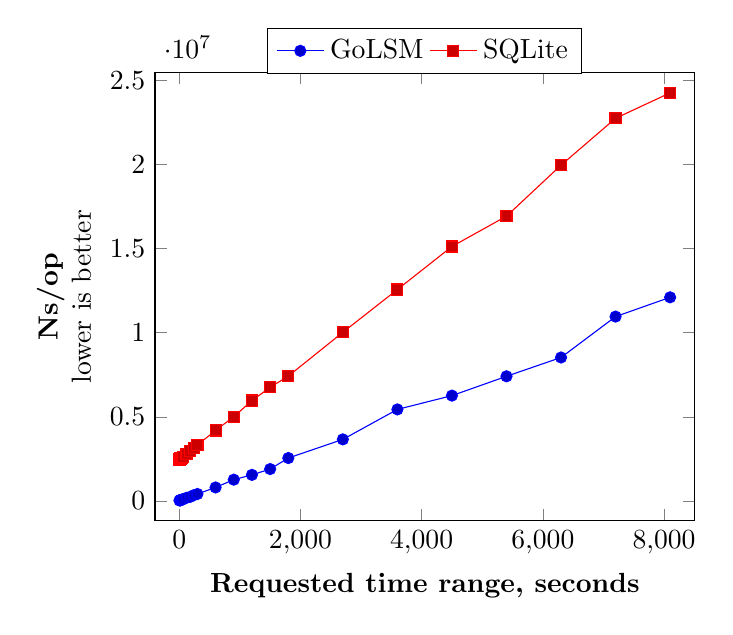
\begin{tikzpicture}
        % first provide your data as table, so later the data can
        % easily be accessed for various stuff
        \pgfplotstableread{
            x    y  z
5 29245				    2468624
10 34331			    2488443
15 41885			    2487442
20 47359			    2533488
25 51261			    2517353
30 62037			    2529031
45 76538			    2571565
60 101490			    2611909
120 185574			    2787438
180 241142			    2986666
240 341329			    3155070
300 412849			    3327132
600 801901			    4190652
900 1264738			    5008636
1200 1549898			    5966411
1500 1895210			    6753930
1800 2550300			    7420697
2700 3659991			    10027510
3600 5442224			    12570023
4500 6261830			    15128483
5400 7410561			    16932040
6300 8529041			    19965360
7200 10960360			    22752193
8100 12106688			    24262132
        }{\data}
    \begin{axis}[
        x tick style={/pgf/number format/1000 sep=},
	    ylabel style={align=center},	
	    ylabel = \textbf{Ns/op}\\lower is better,
	    xlabel style={align=center},	
	    xlabel = \textbf{Requested time range, seconds},
	    enlargelimits=0.05,
	    legend style={
	        at={(0.5,1.1)}, anchor=north,legend columns=-1
	    },
    ]
        % then your `\addplot commands change to
        \addplot table [x=x,y=y] {\data};
        \addlegendentry{GoLSM}
        \addplot table [x=x,y=z] {\data};
        \addlegendentry{SQLite}
    \end{axis}
\end{tikzpicture}